 %!TEX root = main.tex
\chapter{Differential equations in physics and biology}

Most laws of physics and mathematical models of biology are formulated as differential equations.
While these descriptions are often abstract and solving them can be complicated, differential equations are a very natural and intuitive way of describing the world.
The type of differential equations we will consider describe how the state of a system changes over time.

Fig.~\ref{fig:ode} shows two simple settings that can readily described by ordinary differential equations (ODEs).
In the first case, we consider a bucket into which water is flowing at a rate of 10 ml/s.
Clearly, the water level will go up over time and we already know the answer to this problem.
If the water level is initially at time $t_0$ at $y(t_0)=y_0$, at time $t$ it will be given by
\begin{equation}
y(t) = y_0 + 10\frac{ml}{s}\times (t - t_0)
\end{equation}
This is the solution to the differential equation
\begin{equation}
    \frac{dy}{dt} = 10\frac{ml}{s} \, ,
\end{equation}
which is the mathematical equivalent to ``the water increases by 10 milliliter per second''.
The notation $dy$ and $dt$ indicates the limit of small changes $\Delta y$ of $y$ over a small time interval $\Delta t$.

There are two things to note here
\begin{itemize}
    \item the differential equation doesn't specify the initial condition $y_0$. It is valid for any $y_0$.
    \item $y$ describes the water level and is measured in $ml$. The dimensions on both sides of the equation match: $\frac{dy}{dt}$ has units $ml/s$ since $dt$ is a time measured in seconds.
\end{itemize}

\begin{figure}[tb]
    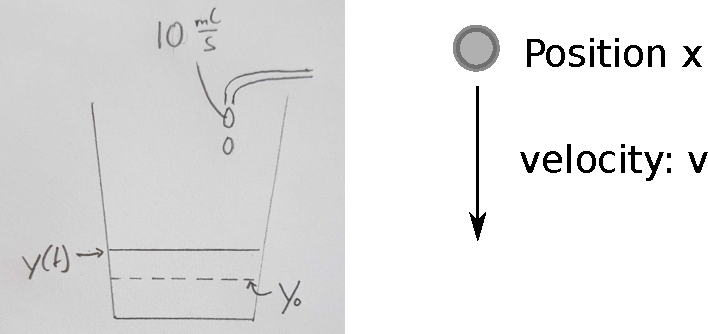
\includegraphics[width=0.8\textwidth]{figures/ODE.pdf}
    \caption{\label{fig:ode} Simple settings that are naturally described by an ordinary differential equation. Left: our simple bucket analogy. Right: a particle moving with velocity $v$.}
\end{figure}

Since differential equations describe how quantities are changing, we can calculate the quantity at a future time point by summing up the changes over time.
In a single time step $\Delta t$ the water level changes as
\begin{equation}
    \label{eq:ODE_step}
    y(t_0 + \Delta t) = y(t_0) + \Delta t \alpha
\end{equation}
where we used the symbol $\alpha$ to denote the influx rate that was 10 ml/s above.
Adding many contributions from such little steps, we can calculate the level at time $t$:
\begin{equation}
    y(t) = y(t_0) + \sum_{i=0}^n \Delta t \alpha
\end{equation}
where $\Delta t = (t-t_0)/n$, that is we split the interval $t-t_0$ into $n$ little steps.
Note that in the above equation, the rate $\alpha$ could change over time:
\begin{equation}
    y(t) = y(t_0) + \sum_{i=0}^n \Delta t \alpha(t_0 + i\Delta t)
\end{equation}
By making $n$ larger and $\Delta t$ smaller, we arrive at an integral over $t'$ from $t_0$ to $t$:
\begin{equation}
    y(t) = y(t_0) + \int_{t_0}^t \alpha(t')\, dt'
\end{equation}

So far, this example has been simple enough that we knew the solution to problem from the beginning and the formalism of ODEs might seem unnecessary.
But let's make this problem slightly more complex and assume the bucket is leaking and the amount of water that leaks is proportional to the pressure and thus to the water level $y(t)$ itself.
In other words, the bucket looses water at a rate $\beta y(t)$, where $\beta$ is the leakage rate.
This additional ``process'' (the leak) can be easily added to the differential equation:
\begin{equation}
    \label{eq:bucket}
    \frac{dy}{dt} = \alpha - \beta y(t)
\end{equation}
The solution to this equation is not quite as easy to guess, but the equation tells us a lot about the system.
The left panel of Fig.~\ref{fig:fixed_points} shows the right hand side of this equation (the rate of change of $y$) as a function of $y$.
For $y<\alpha/\beta$, the influx $\alpha$ is bigger than the leak $\beta y$ and the water level $y$ increases.
Otherwise, the leak is bigger than the efflux and $y$ decreases.
Thus from both sides, the system is driven against $y^* = \alpha/\beta$, which is a \textbf{stable fixed point} of the system.

\begin{figure}
    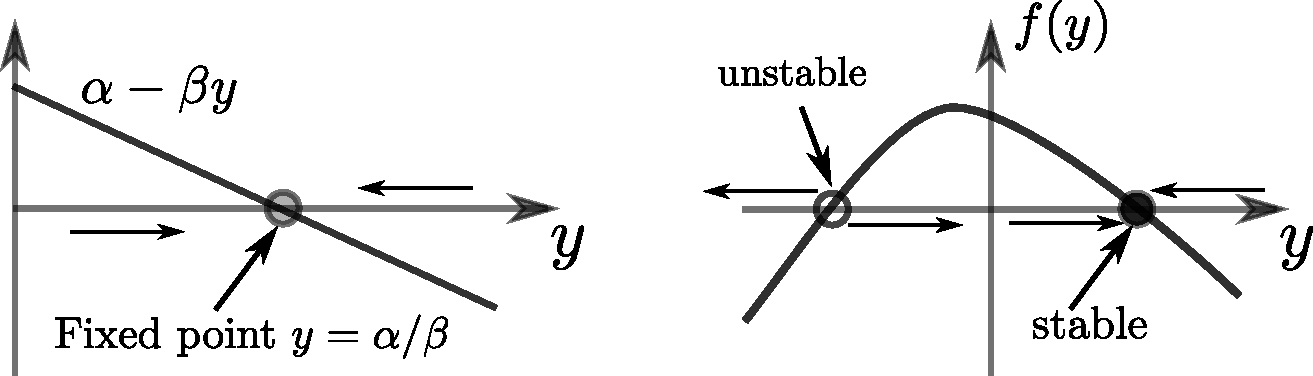
\includegraphics[width=0.8\textwidth]{figures/fixed_points.pdf}
    \caption{\label{fig:fixed_points}Left: Summary of the dynamics of the ODE in Eq.~\ref{eq:bucket}. Right: Stable and unstable fixed points of a generic time independent one dimensional dynamical system.}
\end{figure}

The qualitative analysis above has characterized the most important aspects of the system without actually solving the ODE.
There are many methods for solving ODEs explicitly, but often analysis like the one above or numerical solutions (discussed below) are more useful.
In this case, the system (`leaky bucket') has the solution
\begin{equation}
    y(t) = y_0 e^{-\beta t} + \frac{\alpha}{\beta}\left(1 - e^{-\beta t}\right)
\end{equation}
The initial condition $y_0$ and any deviation from the fixed point decay exponentially with rate $\beta$.
The correctness of this solution can be confirmed by differentiation.

\section{Numerical solutions of differential equations}
Eq.~\ref{eq:ODE_step} describes how the quantity $y$ changes in a small discrete time step $\Delta t$.
Numerical solutions of ODEs work essentially like this: adding small little increments to the solution until time has advanced sufficiently.
\begin{minted}{python}
    y, t = y0, t0            # define initial condition
    tmax, dt = 10, 0.1       # define final time and time step
    while t<tmax:            # loop until tmax and increment t and y
        t += dt
        y += dt*(alpha - beta*y)
\end{minted}
After this code has executed, $y$ will be the approximate solution of Eq.~\ref{eq:bucket}.
The smaller we choose $dt$, the more accurate the solution will be.
This method to solve the equation is often called the ``forward Euler'' method.
It is the simplest, and least accurate, method to solve differential equations.
For our purposes, it will often be good enough.
More complex methods are implemented in libraries which we will explore later in the course.
Please have a look at the accompanying notebooks for code and examples on these numerical solutions.

\section{Motion of particles and Newton's law}
Newton's law of motion
\begin{equation}
    F = m\times a
\end{equation}
is a differential equation. The acceleration $a$ is the rate at which the velocity changes.
The velocity $v$ is the rate at which the position $x$ of a particle changes.
Newton's law is thus not just one, but two coupled differential equations
\begin{equation}
    \begin{split}
        \frac{dx}{dt} & = v \\
        \frac{dv}{dt} & = a = \frac{F}{m} \\
    \end{split}
\end{equation}
The force $F$ can take different form in different problems.

A constant force, for example gravitational force, results in a steadily increasing velocity $v = \frac{Ft}{m}$ (exactly like the bucket without a leak).
This means the position is changing faster and faster with time
\begin{equation}
    \frac{dx}{dt} = \frac{Ft}{m}
\end{equation}
You can readily verify that the solution to this is $x(t) = x_0 + \frac{Ft^2}{2m}$.

Under the gravitational force of the earth, $F = m g$ where $g = 9.81 m/s^2$ and we obtain the familiar results $x(t) = x_0 = \frac{g ^2}{2}$. Note that the mass $m$ cancels.

\subsection{Harmonic oscillator}
Now consider a particle attached to a spring such that the force acting on the particle is $F = -\gamma x$.
This means that for $x>0$, the force is pulling to the left (towards smaller $x$) and in the opposite direction for $x<0$.
Such a situation is similar to a pendulum, a marble in a bowl, or a particle in a laser trap (optical tweezer) used for single molecule experiments (see Fig.~\ref{fig:harmonic}).
In addition to this force acting on the particle, there might also be a friction force.
Friction is typically proportional to the velocity itself $\eta v$.
Combining these two contributions, we find that this system is described by
\begin{equation}
    \label{eq:harmonic}
    \begin{split}
        \frac{dx}{dt} & = v \\
        \frac{dv}{dt} & = -\frac{1}{m} \left( x\gamma +  \eta v\right)\\
    \end{split}
\end{equation}
This system of equations can be solved exactly, but we will explore the solution numerically instead.
This numerical solution can be down for two variables $x$ and $v$ just like we did it for one variable above, see notebooks for details and Fig.~\ref{fig:harmonic} for the result.

The solution in Fig.~\ref{fig:harmonic} shows the trajectories for different levels of friction $\eta$.
This friction is one of the main aspects in which dynamics of large bodies differ from biological system at the micrometer scale.
For the motion of planets, friction can be neglected.
For everyday objects, friction is important, but often a perturbation rather than the dominating force. Nevertheless, objects tend to come to a resting states eventually due to friction.
The smaller the objects, the smaller their mass and friction becomes more important.
With increasing friction, the harmonic oscillator goes from eternal oscillations, to decaying oscillations, to a very slow relaxation.

\begin{figure}
    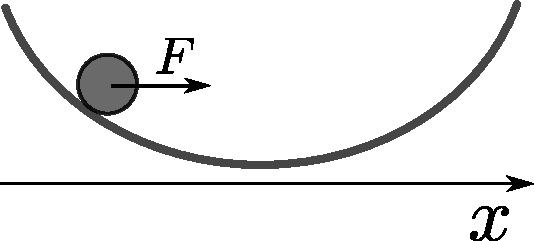
\includegraphics[width=0.4\textwidth]{figures/harmonic.pdf}
    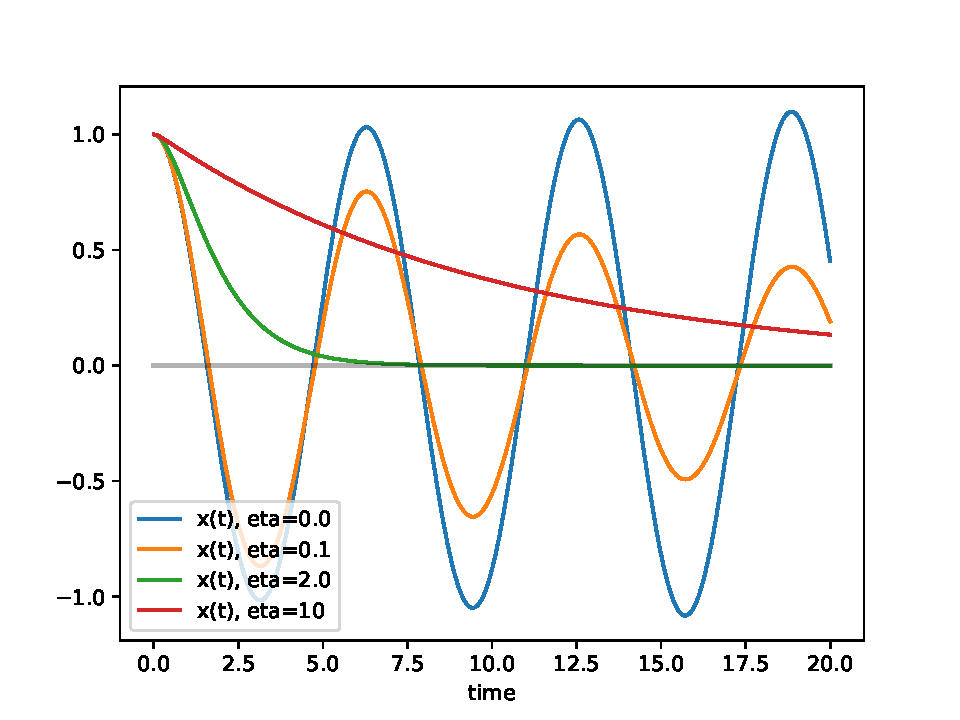
\includegraphics[width=0.55\textwidth]{figures/harmonic_traj.pdf}
    \caption{\label{fig:harmonic}Left: Sketch of a particle moving along direction $x$ in a harmonic potential. Right: Trajectories of the particle at different levels of friction $\eta$.}
\end{figure}


\subsection{Over-damped dynamics}
On the micrometer scale, masses are tiny and friction is typically completely dominating the dynamics.
To explore the consequences of this observation, let's rewrite the second part of Eq.\ref{eq:harmonic} (with $F=-\gamma x$) by multiplying both sides by the mass $m$:
\begin{equation}
    m\frac{dv}{dt} = F - \eta v
\end{equation}
For very small $m$, the left hand side is close to $0$ and hence it follows that the velocity is $v \approx F/\eta$.
In other words, the velocity is the instantaneous ratio of force and friction.
In this over-damped limit, the equation of motion simplfies to
\begin{equation}
    \frac{dx}{dt} = \frac{F}{\eta} = -\frac{\gamma x}{\eta}
\end{equation}
whose solution is a simple exponential decay $x(t) = x_0 e^{-t \gamma/\eta}$.

\subsection{Friction and Stokes' law}
\label{sec:stokeslaw}
Friction in liquid medium is determined by the viscosity of the medium.
Viscosity is something we understand well from everyday life (water, oil, honey all have clearly different viscosity).
For the precise definition of viscosity, one usually considers the configuration in Fig.~\ref{fig:viscosity}.
The force required to move the plate is proportional to their area $A$ and the velocity gradient $v/d$ between the plates.
The constant of proportionality defines the viscosity
\begin{equation}
    F \sim \frac{Av}{d}  \quad \Rightarrow \quad F  = \eta \frac{Av}{d}
\end{equation}
Viscosity has dimension
\begin{equation}
    [\eta] = \left[ \frac{Fd}{Av}\right] = \frac{energy \times time}{volume} = \frac{force \times time}{area}
\end{equation}

Viscosity is typically measured in $N s/m^2$ and relevant values for us are
\begin{itemize}
    \item water: $0.001 \frac{Ns}{m^2}$
    \item cytosol: $0.003 \frac{Ns}{m^2}$
\end{itemize}



\begin{figure}
    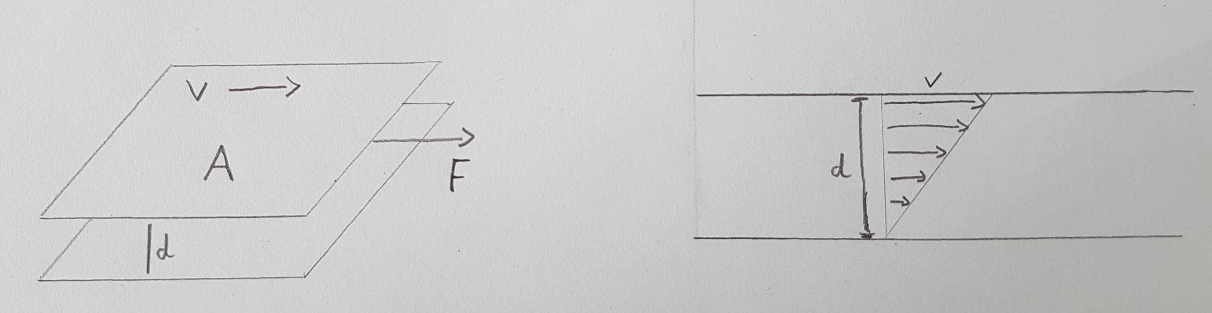
\includegraphics[width=\textwidth]{figures/viscosity.png}
    \caption{\label{fig:viscosity}Viscosity is defined via the force required to move two plates with area $A$ at distance $d$ relative to each other with velocity $v$.}
\end{figure}

\section{Growth processes in biology}

\subsection{Exponential Growth}
see notebooks

\subsection{Logistic Growth}
see notebooks

\subsection{Ecological dynamics}
see notebooks

\subsection{Infectious disease dynamics}
see notebooks


